\section{Addierer}
\label{sec:grundlagen_add}

Die modulare 32-Bit Addition ist die am häufigsten verwendete Operation in der Kompressionsfunktion von \glos{sha256} (Kapitel \ref{chp:sha256}).
Im Gegensatz zu den anderen verwendeten Operationen ist die Addition nicht direkt durch grundlegende binäre Operationen wie AND, OR und XOR definiert.
Die Realisierung bleibt dem Programmierer/Konstrukteur überlassen. Um eine Auswahl zu treffen, werden einige Konstruktionen kurz erläutert.
\begin{description}
  \item[Der Carry-Ripple Addierer] realisiert die Addition mit Hilfe der Schulmethode. Jede Stelle der Binärzahl wird einzeln addiert wobei der Übertrag bei der nächsten
                                   Addition berücksichtigt wird. Durch dieses Vorgehen ist eine Parallelisierung der einzelnen Additionen nicht möglich, da jede
                                   Addition vom Übertrag der vorhergehenden Addition abhängig ist.
  \item[Der Conditional-Sum Addierer] verwendet genau wie der Carry-Ripple Addierer Überträge. Jedoch werden alle Teilsummen zwei Mal berechnet. Einmal mit der Annahme,
                                      dass ein Übertrag vorliegt und einmal ohne. Dadurch können die einzelnen Additionen parallel durchgeführt werden. Abschließend
                                      werden die Teilsummen mit den jeweils korrekten Annahmen zusammengeführt.
  \item[Der Carry-Lookahead Addierer] vermeidet die Abhängigkeit vom Übertrag indem die vorhergehenden Stellen direkt betrachtet werden. Liegt in jeder vorhergehenden
                                      Stelle der Summanden eine $1$ vor (XOR) kann ein generierter Übertrag bis zur aktuellen Addition propagiert werden. Generiert wird
                                      ein Übertrag entweder durch eine direkte Eingabe oder das Vorliegen von zwei $1$en (AND) an einer Stelle der Summanden. Die Betrachtung
                                      der vorhergehenden Stellen und die einzelnen Additionen können dabei parallel durchgeführt werden.
\end{description}
Interessant sind die unterschiedlichen Konstruktionen besonders für die Umsetzung in Hardware. Dort kann eine Beschleunigung der Berechnung durch Parallelisierung
ausgenutzt werden. Während in der Hardware Parallelisierung bedeutet, eine Berechnung mehrfach auf dem Chip unterzubringen, müssen bei einer Realisierung in Software
entsprechend viele Recheneinheiten vorhanden sein. Das macht die 

In dieser Arbeit wird der Carry-Ripple Addierer verwendet, da es sich um eine Umsetzung in Software handelt. Die anderen beiden Konstruktionen 

~\\
Modell des Carry-Ripple Addierers.\\
bezieht alle carry bits mit ein : ermöglicht aussagen über carrys.\\
wichtig für analyse. ein carry auf 0 setzen bedeutet addierer teilen.\\
ein bit vor diesem carry kann sich hinter einem carry 0 nicht mehr auswirken\\
ansonsten kann ein ein einzelnes bit auswirkung auf alle folgebits haben\\
dafür ist nur ein 1 Bit an jeder stelle notwendig\\
~\\
surjective abbildung, jede summe kann aus $2^n$ verschiedenen summanden gebildet werden.\\
umkehrung deshalb nicht eindeutig: gut für cryptography
~\\
Berücksichtigt Carry in und Carry out\\
beides nicht notwendig: Modulo 32 Addierer\\
setzt sich zusammen aus Halbaddierer, Volladdierer und Mod 2 Addierer: xor\\
~\\
Alle 3 vorstellen mit Zeichung \ref{fig:halfadder} \ref{fig:fulladder} \ref{fig:lastadder}

\begin{figure}[!h]
  \centering
  \includegraphics[scale=1]{images/halfadder}
  \caption[Halbaddierer]{Halbaddierer\protect\footnotemark}
  \label{fig:halfadder}
\end{figure}
\footnotetext{Von MovGP0, CC BY-SA 2.0 de, \url{https://commons.wikimedia.org/w/index.php?curid=22912775}}

\begin{figure}[!h]
  \centering
  \includegraphics[scale=1]{images/fulladder}
  \caption[Volladdierer]{Volladdierer\protect\footnotemark}
  \label{fig:fulladder}
\end{figure}
\footnotetext{Von MovGP0, CC BY-SA 2.0 de, \url{https://commons.wikimedia.org/w/index.php?curid=22912742}}

\begin{figure}[!h]
  \centering
  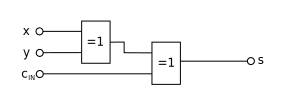
\includegraphics[scale=1]{images/lastadder}
  \caption[Mod-2 Addierer]{Mod-2 Addierer\protect\footnotemark}
  \label{fig:lastadder}
\end{figure}
\footnotetext{Auf Basis von MovGP0, CC BY-SA 2.0 de, \url{https://commons.wikimedia.org/w/index.php?curid=22912742}}

\TODO{erledigen}